\section{Implementation}

\fu{stopped!}
\subsection{Overview}
We propose a strategy to optimize MPC programs and a method to guarantee and verify the information leakage.
Figure \ref{workflow} shows the position of our method in MPC program development workflow.


\begin{figure}[ht]
    \centering
    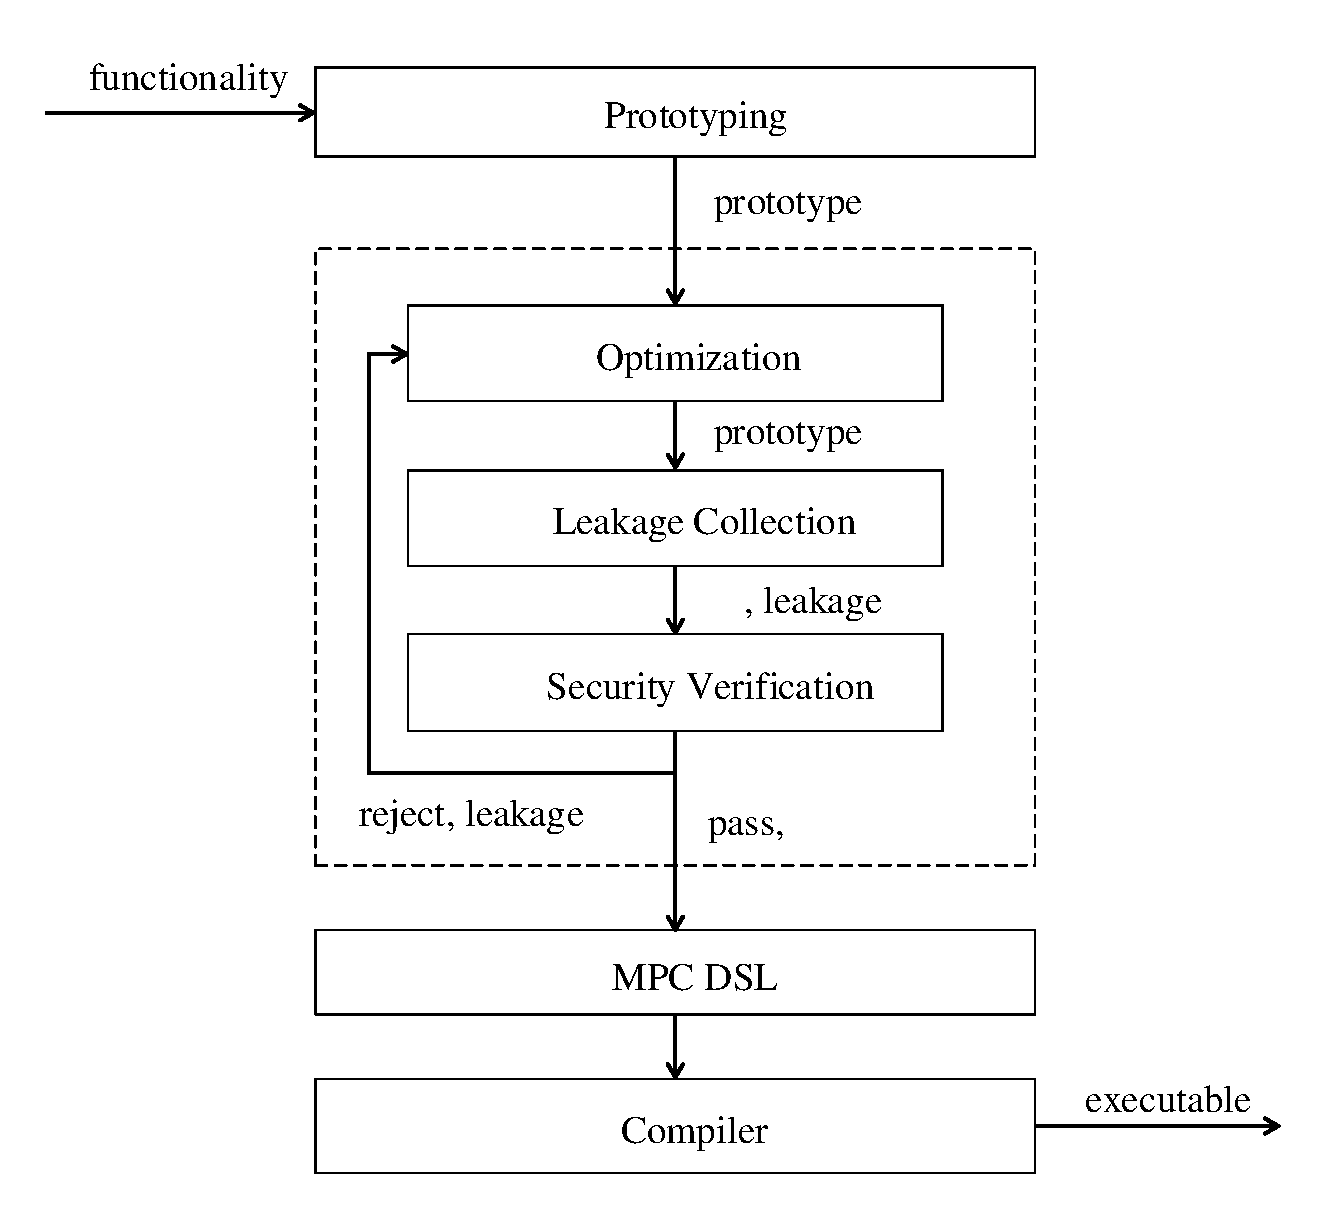
\includegraphics[scale=0.4]{img/workflow.pdf}
    \caption{MPC program development workflow with optimization and verification}
    \label{workflow}
\end{figure}
Our work introduces three parts in the workflow: Optimization, Leakage Collection, and Security Verification.
The optimization part receives a program prototype $p$ which implements the specification including inputs, outputs, functionality $f$ and the \textit{reveal} behavior.
% Programmers reveal some of the intermediate variables in $p$ to reduce the use of oblivious control structures according to our strategy in the optimization part.
The result of the optimization part is $p'$ which is the optimized variant of $p$.
We assume that both $p$ and $p'$ are well-written.
The leakage collection part extracts leakage traces about $p'$ which is modeled in the semantic.
The security verification part verifies the information leakage security of the optimized prototype program $p'$.
The optimized prototype $p'$ will be implemented to practical MPC program if it is secure.
Otherwise, optimized $p'$ has information leakage. Programmers should back to the optimization part and try other optimization.
The complete algorithm of the whole process is as follows \ref{whole}:
\begin{algorithm}[ht]
    \label{whole}
    \caption{Overview}
    \begin{algorithmic}
    \Require Program $p$
    \Ensure $p'$ is leakage secure
    \State log = None
    \While {True}
        \State $p'$ = Optimization($p$, log)
        \State $\Phi$ = Collector($p'$)
        \State secure, log = Verification($p'$, $\Phi$)
        \If {secure}
            \State \Return $p'$
        \EndIf
    \EndWhile
    \end{algorithmic}
\end{algorithm}

\subsection{Optimization}
A straightforward way to improve the performance of MPC program is to reduce the gates of the circuit required by evaluating the MPC program.
According to our observation of MPC, revealing some of the intermediate variables can reduce the use of oblivious control structures so that reduce the size of the circuit.
At the same time, the security is not weakened by the appropriate selection of the intermediate variables to be revealed to ensure that no information leakage is caused.

In the language model in Figure \ref{syntax} and \ref{semantic}, the above strategy is achieved by revealing the oblivious condition variable of obliv if-statement and transferring the obliv if-statement to an if-statement.
The performance of MPC protocols in the real world depends on various factors such as protocol type, CPU performance, network bandwidth, and network latency, so we cannot give a universal optimal strategy.
We allow programmers to transform arbitrary obliv if-statements of a program to if-statements.
The next two parts guarantee the information leakage of the optimized program by verification.

\subsection{Leakage Collection}
We have modeled the information leakage of MPC programs in Section \ref{preli}.
We use a symbolic execution-based approach to extract leakage from MPC programs.
The Algorithm \ref{collect} shows the skeleton of our leakage collector.
The collector extracts leakage trace and leakage lower bound from program $p$.
Algorithm \ref{collect} interprets program $p$ on symbolic memory $\sigma$.
Leakage trace $\phi$ is a sequence of information leakage of an execution path.
$\Phi$ is the set of all leakage traces. $\Phi[\MPCState{y}{\sigma}]$ is the sequence of leakage trace $\phi$ of execution paths whose result is $\MPCState{y}{\sigma}$.
$\Psi$ is the leakage lower bound which is in constraint form in the algorithm.
$\Psi[\MPCState{y}{\sigma}]$ build the constraint for equivalence class $[\thicksim_l]$ where $l=\textit{Eq}(expr_y, \MPCState{y}{\sigma})$.
\begin{algorithm}
    \label{collect}
    \caption{Collector }
    \begin{algorithmic}
    \Require Program $p$, Symbolic memory $\sigma$, Leakage $\phi$, $\psi$
    \Ensure Leakage trace set $\Phi$, Leakage lower bound $\Psi$
    \If {$\MPCAngle{p}$ == $\MPCAngle{\text{skip}}$}
        \State $\Phi$[$\MPCState{y}{\sigma}$].append($\phi$)
        \State $\Psi$[$\MPCState{y}{\sigma}$] =  $\Psi$[$\MPCState{y}{\sigma}$] $\lor$ $\psi$
    \ElsIf{$\MPCAngle{p}$ == $\MPCAngle{\text{skip};p_1}$}
        \State Collector($p_1,\sigma, \phi$)
    \ElsIf {$\MPCAngle{p}$ == $\MPCAngle{lv = e;p_1}$}
        \State Collector($p_1,\sigma[lv\mapsto \MPCState{e}{\sigma}], \phi$)
    \ElsIf {$\MPCAngle{p}$ == $\MPCAngle{lv = \textit{reveal } e;p_1}$}
        \State $\phi$.append($\textit{Eq}(expr_{lv},\MPCState{e}{\sigma})$)
        \State Collector($p_1,\sigma[lv\mapsto \MPCState{e}{\sigma}], \phi$)
    \ElsIf {$\MPCAngle{p}$ == $\MPCAngle{\text{[Obliv] if } e \text{ then } p_1 \text{ else } p_2;p_3}$}
        \State $\psi$.append($\textit{Eq}(expr_{e},\MPCState{e}{\sigma})$)
        \If { SAT$(\MPCState{e}{\sigma})$  }
            \State Collector($p_1;p_3, \sigma, \phi$)
        \EndIf
        \If { SAT$(\MPCState{\text{not }e}{\sigma})$}
            \State Collector($p_2;p_3,\sigma, \phi$)
        \EndIf
    \ElsIf {$\MPCAngle{p}$ == $\MPCAngle{\text{while } e \text{ do } p_1 ; p_2}$}
        \State $\psi$.append($\textit{Eq}(expr_{e},\MPCState{e}{\sigma})$)
        \If {SAT$(\MPCState{e}{\sigma})$}
            \State Collector($p_1;\text{while } e \text{ do } p_1; p_2,\sigma,\phi$)
        \Else {}
            \State Collector($p_2;\sigma,\phi$)
        \EndIf
    \EndIf
    \State \Return $\Phi$, $\Psi$
    \end{algorithmic}
\end{algorithm}
\subsection{Security Verification}
The security should ensure that the leakage of the optimized MPC program $p^\prime$ within the leakage lower bound of the standard MPC program $p$.
The optimized program $p'$ has the same functionality as the standard program $p$.
As we discussed, the leakage lower bound comes from the revealed oblivious result.
Thus, $p$ and $p'$ has the same leakage lower bound.
\begin{theorem}
    MPC programs $p$ and $p'$ have the same leakage lower bound $\Psi$ if they have the same functionality $f$.
\end{theorem}
\begin{proof}
    With the same assumption of private inputs, $p$ has leakge lower bound $\Psi$ and $p'$ has leakage lower bound $\Psi'$.
    Suppose that $\Psi$ and $\Psi'$ are different, then the equivalence class partition of private inputs of $p$ and $p'$ are different.
    The partition is the mapping from private inputs to results, which is exactly the mapping of functionality $f$.
    It contradicts that $p$ and $p'$ have the same functionality $f$.
\end{proof}
\begin{theorem}(Leakage security)
    The leakage of $p'$ is $\Psi^\prime$ and the leakage lower bound of $p'$ is $\Psi$, $p'$ is leakage secure if $\Psi \equiv \Psi'$.
\end{theorem}

\begin{corollary}
    For program $p'$ with private input $x\in X$ and result $y\in Y$, $\Psi \equiv \Psi'$ if and only if $\forall y: \Psi_{y}\equiv\Psi_{y}'$.
\end{corollary}

\begin{corollary}
    For program $p'$ with private input $x\in X$ and result $y\in Y$,
    $\Psi_y \equiv \Psi_y'$ if and only if $\forall \phi\in \Phi[y]: \Psi_{y}\equiv\Psi_{y}\land \phi $.
\end{corollary}

Simplify the condition as:
\begin{equation}
    \begin{split}
    &\Psi_y \equiv \Psi_y' \\
    \Leftrightarrow & \forall{\phi\in \Phi[y]}: \Psi_y \equiv \Psi_y\land \phi  \\
    \Leftrightarrow & \forall{\phi\in \Phi[y]}: \neg (\Psi_y \oplus (\Psi_y\land \phi ))\\
    \Leftrightarrow & \forall{\phi\in \Phi[y]}: \neg (\Psi_y \land (\neg \Psi_y \lor \neg \phi)) \\
    \Leftrightarrow & \forall{\phi\in \Phi[y]}: \neg \Psi_y \lor \phi \\
\end{split}
\end{equation}
As we verify the partition of case $y$, the $\Psi_y$ holds. So:
\begin{equation}
    \label{simend}
    \begin{split}
    &\Psi_y \models  \forall{\phi\in \Phi[y]}: \neg \Psi_y \lor \phi \\
    \Leftrightarrow & \Psi_y \models \forall{\phi\in \Phi[y]}: \phi \\
    \Leftrightarrow & \Psi_y \models \bigwedge_{\phi\in \Phi[y]} \phi \\
\end{split}
\end{equation}
For each constraint of $\Psi$, we verify the condition in Eq. \ref{simend} to ensure that the partition corresponding to this constraint holds in $p'$.
The algorithm of verification process is in Algorithm \ref{algo-verify}.
\begin{algorithm}
    \label{algo-verify}
    \caption{Verification }
    \begin{algorithmic}
    \Require Leakage lower bound $\Psi$, Leakage trace $\Phi$
    \Ensure Pass or Reject
    \State log = None
    \For {each $y \in Y$}
        \State b = Solver($\Psi_y \models \bigwedge_{\phi\in \Phi[y]} \phi$)
        \If {$\neg$b}
            \State \Return Reject
        \EndIf
    \EndFor
    \State \Return Pass
    \end{algorithmic}
\end{algorithm}

% \begin{proof}(Soundness)
%     For program $p'$ with private input $x\in X$ and result $y\in Y$,
%     When $p'$ pass verification process, we have $y\in Y$, $\Psi_y \equiv \Psi_y'$ for any $y$.
%     Thus, $\Psi \equiv\Psi'$, $p'$ is leakage secure.
% \end{proof}

\begin{theorem}(Semi-honest security)
    For program $p$ with private input $x\in X$ and result $y\in Y$, suppose $p$ has leakage $\Psi$ and is secure against a semi-honest adversary.
    For program $p'$ with private input $x\in X$ and result $y\in Y$, if $p'$ has information leakage $\Psi$, $p'$ is secure against the semi-honest adversary.
\end{theorem}
\begin{proof}
\textit{sketch.}
In the ideal world, the simulator knows the partition corresponding to the private inputs.
Suppose $TTP$ in the ideal world gets result $y$. The simulator knows that the constraint is $\Psi_y$.
During the simulation of $View_{\text{sim},adv}^{p'}$, each time a intermediate variable $v$ are revealed, the simulator check the satisfiable of $\Psi_y\land Eq(expr_v, true)$.
If so, the simulator send a message such that the decrypt of $v$ is true. Otherwise, the simulator send a massage such that the decrypt of $v$ is false.


Consider the ideal world vs. real world paradigm of program $p$, the adversary's view in the real world is $View_{\text{real},adv}^{p}$ , in the ideal world is $View_{\text{sim},adv}^{p}$. $p$ is secure against the semi-honest adversary, so the distributions of $View_{\text{real},adv}^{p}$  and $View_{\text{sim},adv}^{p}$ are indistinguishable to the adversary. For program $p'$, suppose the distributions of $View_{\text{real},adv}^{p'}$  and $View_{\text{sim},adv}^{p'}$  are distinguishable. The adversary has to obey the protocol to execute $p'$ without any active behavior such as interrupt the protocol, send spurious messages and so on. In this situation, The difference between $View_{adv}^{p'}$ and $View_{adv}^{p}$ is the revealed control flow information $\psi_e$ for each execution. The view of $\psi_e$ for the distribution of $View_{adv}^{p'}$ is the combination form $\bigwedge_{pt}\psi_{pt}$. Thus, $View_{adv}^{p'}$ becomes distinguishable due to the knowledge $\bigwedge_{pt}\psi_{pt}$. However, we have proved that $ \neg \Psi_y \lor \bigwedge_{pt\in Path(y)} \psi_{pt}\Leftrightarrow\Psi_y\rightarrow \bigwedge_{pt\in Path(y)}\psi_{pt}$ , and $\Psi$ is also learnt from $View_{adv}^{p}$. Thus, $View_{adv}^{p}$ is distinguishable. However, it is contradict to the assumption that $p'$ is secure against the semi-honest adversary. Therefore, $View_{\text{real},adv}^{p'}$ and $View_{\text{sim},adv}^{p'}$ are indistinguishable, and $p'$ is secure against the semi-honest adversary.
\end{proof}
